\documentclass[11pt]{report}
\usepackage{amsmath, amsthm}
\usepackage[pdftex]{graphicx}
\usepackage{psfrag,epsf}
\usepackage{enumerate}
\usepackage{natbib}
\usepackage{float}
\restylefloat{table}

\usepackage{amssymb}
\usepackage{multirow}
\usepackage{float}

\usepackage{Sweave}
\begin{document}
\Sconcordance{concordance:icenReg.tex:icenReg.Rnw:%
1 13 1 1 0 635 1}


\title{Using {\bf{icenReg}} for interval censored data in {\bf{R} } }
\author{Clifford Anderson-Bergman}
\maketitle


\tableofcontents

\chapter{Introduction}

  \section{Interval Censoring}

  Interval censoring occurs when a response is known only up to an interval. 
  A classic example is testing for diseases at a doctor's clinic; if a 
  subject tests negative at $t_1$ and positive at $t_2$, all that is known is
  that the subject acquired the disease in ($t_1$, $t_2$), rather than an exact time. 
  Other classic examples include examining test mice for tumors after sacrifice 
  (results in \emph{current status} or \emph{case I} interval censored data, in which
  all observations are either left or right censored, as opposed to the more general
  \emph{case II}), customer choice models in economics (customers are presented a price
  for a product and chose to purchase or not, researcher wants to know distribution of 
  maximum spending amount; this results in current status data again), 
  data reduction methods for sensor analyses (to reduce load on sensor system, message
  is intentionally surpressed if outcome is in an expected region) and data binning 
  (responses reported only up to an interval, in some cases to keep the subjects
  anonymous, in some cases to reduce size of data). 

  
  Often interval censoring is ignored in analysis. For example, age is usually reported only 
  up to the year, rather than as a continuous variable. In the case that these intervals
  are relatively short, the bias introduced by ignoring the interval censoring may be 
  small enough to be safely ignored. However, in the case that the width of intervals is non
  trivial, statistical methods that account for this should be used for reliable analysis. 
  
  \section{Classic Estimators}
  
  The topic of interval censoring began emerging in the field of survival analysis. 
  Although it is now considered in other fields of study (such as \emph{tobit regression}),
  at this time {\bf{icenReg}} focusses on survival models. 
  
  
  One of the earliest models is the \emph{Non-Parametric Maximum Likelihood Estimator} 
  (NPMLE), also referred to as \emph{Turnbull's Estimator}. This is a generalization of
  the Kaplan Meier curves (which is a generalization of the empirical distribution function)
  that allows for interval censoring. Unlike the Kaplan Meier curves, the solution is not
  in closed form and several algorithms have been proposed for efficient computation. 
  A special topic regarding the NPMLE is the bivariate NPMLE; this is for the special 
  case of two interval censored outcomes, in which the researcher wants a non-parametric 
  estimator of the joint distribution. This is especially computationally intense as the
  number of parameters can be up to $n^2$. 
  
  Semi-parametric models exist in the literature as well; two classic regression models
  fit by {\bf icenReg} are the Cox-PH model and the proportional odds model. 
  The well known Cox-PH, or proportional hazards regression model, has the property that
  
  \[ h(t | X, \beta) = h_o(t) e^{X^T \beta} \]
  
  where $h(t | X, \beta)$ is the hazard rate conditional on covariates $X$ and regression parameters $\beta$,
  with $h_o$ as the baseline hazard function. This relation is equivalent to 

  \[S(t | X, \beta) = S_o(t)^{e^{X^T \beta} } \]
  
  where $S(t| X, \beta)$ is the conditional survival and $S_o(t)$ is the baseline survival function. 
  
  The less known proportional odds model can be expressed as
  
  \[\text{Odds}(S(t | X, \beta)) = e^{X^T \beta} \text{Odds}(S_o(t)) \]
  \begin{center}  
  or
  \end{center}
  \[ \frac{S(t | X, \beta)} {1 - S(t | X, \beta) } = e^{X^T \beta}\frac{S_o(t)} {1 - S_o(t)} \]
  
  
  Unlike the special example
  of the Cox PH model with right-censored data, the baseline parameters 
  \emph{must} be estimated concurrently
  with the regression parameters. The model can be kept semi-parametric (i.e. no need to 
  decide on a parametric baseline distribution) by using the Turnbull estimator, modified
  to account for the given regression model, as the baseline distribution. 
  The semi-parametric model can be computationally very difficult,
  as the number of baseline parameters can be quite high (up to $n$), which must follow
  shape constraints (i.e. either a set of probability masses or a cumulative hazard function,
  which must be strictly increasing) and there is no closed form solution to either
  regression or baseline parameters.
  
  Fully parametric models exist as well and can be calculated using fairly standard
  algorithms. There are slight complications in that the interval censoring causes the log
  likelihood function to be non-concave. However, only slight modifications are required to 
  adress this issue. In practice, fully-parametric models should be used with caution; the
  lack of observed values means that model inspection can be quite difficult; there are no
  histograms, etc., to be made. As such, even if fully parametric models are to be used for
  the final analysis, it is strongly encouraged to use semi-parametric models at least for
  model inspection. {\bf icenReg} fits both proportional odds and proporitonal hazard models for interval
  censored data. 
  
  Another common regression model for survival data is the accelerated failure time model (AFT).
  At this time, this option is not available for interval censored data. However, this model
  can be fit for interval censored data using {\bf survival}'s \texttt{survreg} function. 
  
\section{Models fit with {\bf{icenReg}} }

  The author's motivation for building {\bf{icenReg}} was to build a set of fast, reliable
  tools for analysts' to use on applied data. At this time, the following set of models can 
  be fit (name in paratheses is function call in {\bf{icenReg}}):
  
  \begin{itemize}
  
    \item NPMLE (\texttt{ic\_sp} can be used to fit univariate NPMLE, alternatively \texttt{ICNPMLE} can be used to fit univariate or bivariate NPMLE)
  
    \item Semi-parametric model (\texttt{ic\_sp}, with options \texttt{model = "ph"} for 
    porportional hazards, \texttt{"po"} for proportional odds)
    
    \item Fully parametric model (\texttt{ic\_sp}, in additon to \texttt{model} option, also 
    have a choice of \texttt{dist}, with options \texttt{"exponential", "gamma", "weibull", "lnorm", "loglogistic" and "generalgamma"})
  
  \end{itemize}
  
  In addition, {\bf{icenReg}} includes various diagnostic tools. These include
  
  \begin{itemize}
  
    \item Plots for diagnosising baseline distribution (\texttt{diag\_baseline})
    
    \item Plots for diagnosising covariate effects (\texttt{diag\_covar})
    
    \item Cross validation via multiple imputations (\texttt{icenReg\_cv})
  
  \end{itemize}
  
  
  \section{Data Examples in {\bf{icenReg}} }
  
  The package includes 4 sources of example data: two functions that simulate data and
  two sample data sets. The simulation functions are \texttt{simIC\_weib}, which simulates
  interval censored regression data with a Weibull baseline distribution and 
  \texttt{simBVCen}, which simulates bivariate interval censored data. The sample data sets
  are \texttt{miceData}, which contains current status data regarding lung tumors 
  from two groups of mice and \texttt{essIncData}, which includes data from the European
  Social Survey. In this case, wages were only recorded up to an interval to 
  protect the identity of the subjects. The dataset \texttt{essIncData\_small} is a smaller
  subset of \texttt{essIncData} (n = 500 instead of 6,712), which is used in many of 
  the examples only so that CRAN's testing of the package runs quicker. In practice,
  using all these models on n = 6,712 is trival to do, rarely taking more than a few seconds
  even on a slower laptop. 
  
  
  \chapter{Fitting Models in {\bf{icenReg}} }
  
  An important note about {\bf icenReg} is that in all models, it is assumed that the 
  response interval is {\bf closed}, i.e. the event is known to have occurred within 
  $[t_1, t_2]$, compared with $[t_1, t_2)$, $(t_1, t_2)$, etc. This is of no consequence 
  for fully parametric models, but does mean the solutions may differ somewhat in 
  comparison with semi- and non-parametric models that allow differnt configurations
  of open and closed response intervals. 
  
  \section{Non-parametric models}
  
  As noted earlier, for univariate interval censored data, the model may be fit with either
  \texttt{ic\_sp} or \texttt{ICNPMLE}. For large datasets (i.e. n > 50,000), \texttt{ic\_sp} 
  will become faster than \texttt{ICNPMLE}. In addition, \texttt{ic\_sp} can readily be 
  provided to the \texttt{plot} method. For bivariate data, \texttt{ICNPMLE} is currently
  the only choice. 
  
  If the data set is relatively small and the user is interested in non-parametric tests,
  such as the log-rank statistic, we actually advise using the {\bf interval} package,
  as this provides several testing functions. However, {\bf icenReg} is several fold 
  faster than {\bf interval}, so if large datasets are used (i.e. n > 1,000), the user
  may have no choice but to use {\bf icenReg}.
  
  To fit an NPMLE model for interval censored data, we will consider the \texttt{miceData}
  provided in {\bf icenReg}. This dataset contains three variables: \texttt{l, u} and
  \texttt{grp}. \texttt{l} and \texttt{u} represent the left and right side of the interval
  containing the event time (note: data is current status) and \texttt{grp} is a group
  indicator with two categories.
  
  If we separate the data into two datasets, i.e. 
  
  \begin{verbatim}
  ge.data <- miceData[miceData$grp == "ge", ]
  ce.data <- miceData[miceData$grp == "ce", ]
  \end{verbatim}

  We can then fit the NPMLE by calling the interval censored semi-parametric model, 
  but supplying no covariates. This can be done by 
  
  \begin{verbatim}
  ge.fit <- ic_sp(cbind(l, u) ~ 0, data = ge.data)
  ce.fit <- ic_sp(cbind(l, u) ~ 0, data = ce.data)
  \end{verbatim}

  Because the objects returned by \texttt{ic\_sp} are intended
  to describe semi-parametric models and thus focus on the 
  regression parameters. For the NPMLE, we need the information
  about the survival curve. 
  We can extract the estimated survival curves by \texttt{getSCurves}
  
  \begin{verbatim}
  ge.sc <- getSCurves(ge.fit)
  ce.sc <- getSCurves(ce.fit)
  \end{verbatim}

  We can then plot and examine the NPMLE's for the two different groups
  using \texttt{plot} and \texttt{lines}
  
  \begin{verbatim}
  plot(ge.sc, xlab = 'Time', 
    ylab = 'Estimated Survival', col = 'blue')
  lines(ce.sc, col = 'red')
  legend('bottomleft', legend = c('ge', 'ce'), 
      col = c('blue', 'red'), lty = 1)
  \end{verbatim}

  \begin{figure}
  \centerline{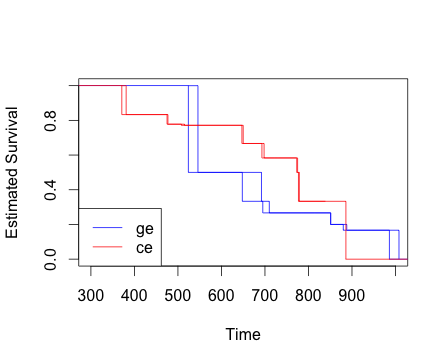
\includegraphics{MICE_NPMLES.png}}
  \caption[MICE NPMLE]{NPMLE's for both groups in miceData} 
  \label{figure:MICE}
  \end{figure}

  Looking at figure \ref{figure:MICE}, we can see a unique feature about the NPMLE for 
  interval censored data. That is, there are \emph{two} lines used to represent
  the survival curve. This is because with interval censored data, the NPMLE
  is not always unique (in fact, it usually is not); any curve that lies between
  the two lines has the same likelihood. For example, any curve that lies between
  the two blues lines in figure \ref{figure:MICE} maximizes the likelihood 
  associated with \texttt{"ge"} group of mice. 

  Formal statistical tests using the NPMLE are not currently supported by 
{\bf icenReg}. We recommend using the {\bf interval} package for this. 

  \section{Semi-parametric models}

  Fitting the semi-parametric models is identical to fitting the non-parametric

\end{document}
